\section{De Giorgi type varifold solutions for mean curvature flow}
\label{subsection_de_giorgi_type_varifold_solutions_for_mcf}

Up until this point, we have always made the crucial assumption of energy 
convergence (\ref{energy_convergence}) for our proofs.
However this is usually a very strong assumption. One thing which could go 
wrong is for example illustrated in 
\Cref{figure_interfaces_collapse}. There we see that two approximate interfaces 
of 
the first and second phase collapse as $ \varepsilon $ tends to zero. This 
results in a loss of energy since the measure theoretic boundary of a set with
finite perimeter does not see such lines.

\begin{figure}[h]
	\centering
	
	\begin{subfigure}[b]{0.3\linewidth}
		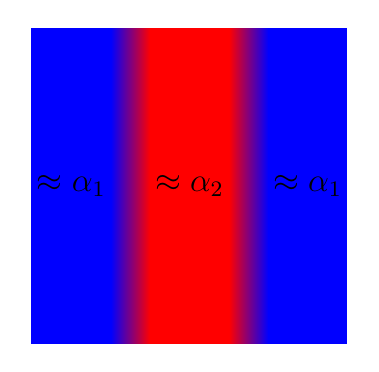
\begin{tikzpicture}
			\filldraw[fill=blue, draw=blue] (0,0) rectangle (1,4);
			\shade[left color=blue,right color=red] (1,0) rectangle (1.5,4);
			\filldraw[fill=red, draw=red] (1.5,0) rectangle (2.5,4);
			\shade[left color=red,right color=blue] (2.5,0) rectangle (3,4);
			\filldraw[fill=blue, draw=blue] (3,0) rectangle (4,4);
			
			\node at (0.5,2) {\large $\approx \alpha_{ 1 } $};
			\node at (2,2) {\large $\approx \alpha_{ 2 } $};
			\node at (3.5,2) {\large $\approx \alpha_{ 1 } $};
			
		\end{tikzpicture}
		
		\caption{$ 1 > \varepsilon > 0 $}
		\label{subfigure_epsilon}
	\end{subfigure}
	\hfill
	\begin{subfigure}[b]{0.3\linewidth}
		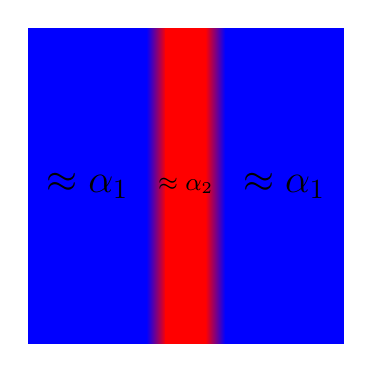
\begin{tikzpicture}
			\filldraw[fill=blue, draw=blue] (0,0) rectangle (1.5,4);
			\shade[left color=blue,right color=red] (1.5,0) rectangle (1.75,4);
			\filldraw[fill=red, draw=red] (1.75,0) rectangle (2.25,4);
			\shade[left color=red,right color=blue] (2.25,0) rectangle (2.5,4);
			\filldraw[fill=blue, draw=blue] (2.5,0) rectangle (4,4);
			
			\node at (0.75,2) {\Large $\approx \alpha_{ 1 } $};
			\node at (2,2) {\small $\approx \alpha_{ 2 } $};
			\node at (3.25,2) {\Large $\approx \alpha_{ 1 } $};
			
		\end{tikzpicture}
		
		\caption{$ 1 \gg  \varepsilon >0 $}
		\label{subfigure_varepsilon_prime}
	\end{subfigure}
	\hfill
	\begin{subfigure}[b]{0.3\linewidth}
		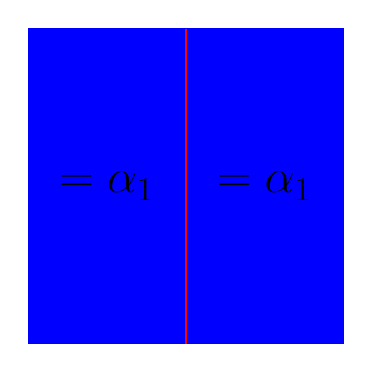
\begin{tikzpicture}
			\filldraw[fill=blue, draw=blue] (0,0) rectangle (4,4);
			\draw[red,thick](2,0)--(2,4);
			
			\node at (1,2) {\LARGE $= \alpha_{ 1 } $};
			\node at (3,2) {\LARGE $= \alpha_{ 1 } $};
			
		\end{tikzpicture}
		
		\caption{$ \varepsilon = 0 $}
		\label{subfigure_varepsilon_zero}
	\end{subfigure}
	
	\caption{Profile of the solution $u_{ \varepsilon } $ as $ \varepsilon $ 
		tends to zero.}
	\label{figure_interfaces_collapse}
\end{figure}

We now introduce the solution concept by Hensel and Laux in 
\cite{hensel_laux_varifold_solution_concept_for_mean_curvature_flow} which 
tackles this issue. 
For the two-phase case, the definition is as follows.

\begin{definition}[De Giorgi type varifold solution for two-phase mean 
	curvature flow]
	\label{de_giorgi_varifold_solution_for_mcf}
	Let $ T < \infty $ be an arbitrary finite time horizon and let $ \mu = 
	\lm^{ 1 } \otimes ( \mu_{ t } )_{ t \in ( 0 , T ) } $ be a 
	family of oriented varifolds $ \mu_{ t } \in \mathcal{ M } \left( 
	\flattorus \times \mathbb{ S }^{ d - 1 } \right) $ for $ t \in ( 0 , T ) 
	$ such that the map $ t \mapsto \int_{ \flattorus \times \mathbb{ S }^{ d 
			-1 } } \eta (t, x , p ) \dd \mu_{ t } ( x , p ) $ is measurable 
			for all 
	$ \eta \in \lp^{ 1 } \left( ( 0 , T ) ; \cont \left( \flattorus, 
	\mathbb{ S 
	}^{ d - 1 } \right) \right) $. 
	Consider also a family $ A = ( A_{ t } )_{ t \in ( 0 , T ) } $ of 
	subsets of $ \flattorus $ with finite perimeter such that the associated 
	indicator function $ \chi ( x , t ) \coloneqq \chi_{ A _{ t } } ( x ) $ 
	satisfies 
	$ \chi \in \lp^{ \infty } \left( ( 0 , T ) ; \bv ( \flattorus ; \{ 0 , 
	1 \} ) \right) $.
	Let $ \sigma > 0 $ be a surface tension constant.
	
	Given an initial energy
	$ \omega^{ 0 } \in \mathcal{ M } \left( \flattorus \right) $ and initial 
	data $ \chi^{ 0 } \in \bv 
	\left( \flattorus ; \{ 0 , 1 \} \right)$, we call the pair $ ( \mu , \chi ) 
	$ a \emph{De Giorgi type varifold solution to two-phase mean curvature 
	flow 
		with initial data} $ ( \omega^{ 0 } , \chi^{ 0 } ) $ if the following 
		holds.
	\begin{enumerate}
		\item (Existence of a normal speed)
		Writing $ \mu_{ t } = \omega_{ t } \otimes ( \lambda_{ t, x } )_{ x 
			\in \flattorus} $ for the disintegration of $ \mu_{ t } $, we 
			require 
		the existence of some 
		$ V \in \lp^{ 2 } \left( ( 0 , T ) \times \flattorus ,
		\omega_{ t } \right) $ encoding a normal velocity in the sense of
		\begin{equation}
			\label{equation_varifold_velocity}
			\sigma
			\int
			\chi ( T' , x ) \varphi ( T' , x ) 
			-
			\chi^{ 0 } ( x ) \varphi (0,x)
			\dd{ x }
			=
			\sigma
			\int_{ 0 }^{ T' }
			\int
			\chi
			\partial_{ t } \varphi 
			\dd{ x }
			\dd{ t }
			+
			\int_{ 0 }^{ T' }
			\int
			V \varphi 
			\dd{ \omega_{ t } }
			\dd{ t }
		\end{equation}
		for almost every $ T' \in ( 0 , T ) $ and all $ \varphi \in \cont_{ 
			\mathrm{c} }^{ \infty } \left( [ 0 , T ) \times \flattorus \right) 
		$.
		
		\item (Existence of a generalized mean curvature vector)
		We require the existence of some 
		$ H \in \lp^{ 2 } \left( 
		( 0 , T ) \times \flattorus , \omega_{ t } ; \mathbb{ R }^{ d } \right) 
		$
		encoding a generalized mean curvature vector by
		\begin{equation}
			\label{equation_varifold_mean_curvature}
			\int_{ 0 }^{ T }
			\int
			\inner*{ H }{ \xi }
			\dd{ \omega_{ t } }
			\dd{ t }
			=
			-
			\int_{ 0 }^{ T }
			\int_{ \flattorus \times \mathbb{ S }^{ d - 1 } }
			\inner*{ \xi }{ \mathrm{Id} - p \otimes p }
			\dd{ \mu_{ t } ( x, p ) }
			\dd{ t }
		\end{equation}
		for all $ \xi \in \cont_{ \mathrm{c} }^{ \infty } \left( [ 0, T ) 
		\times \flattorus ; \mathbb{ R }^{ d } \right) $.
		
		\item (De Giorgi type optimal energy dissipation inequality)
		A sharp energy dissipation inequality holds in form of
		\begin{equation}
			\label{equation_varifold_de_giorgi_inequality}
			\omega_{ T' } ( \flattorus )
			+
			\frac{ 1 }{ 2 }
			\int_{ 0 }^{ T' }
			\int
			V^{ 2 }
			+
			\abs{ H }^{ 2 }
			\dd{ \omega_{ t } }
			\dd{ t }
			\leq
			\omega^{ 0 } ( \flattorus )
		\end{equation}
		for almost every $ T' \in ( 0 , T ) $.
		
		\item (Compatibility)
		For almost every $ t \in ( 0 , T ) $ and all $ \xi \in \cont^{ 
			\infty } \left( \flattorus ; \mathbb{ R }^{ d } \right) $, it holds 
			that
		\begin{equation}
			\label{equation_varifold_compatibility}
			\sigma
			\int
			\inner*{ \xi }
			{ \nabla \chi ( t , \cdot ) }
			=
			\int_{ \flattorus \times \mathbb{ S }^{ d - 1 } }
			\inner*{ \xi }{ p }
			\dd{ \mu_{ t } ( x, p ) }.
		\end{equation}
	\end{enumerate}
\end{definition}

We firstly want to discuss this definition. If we have a De Giorgi type $ \bv 
$-solution $ \chi $ to two-phase mean curvature flow in the sense of 
\Cref{de_giorgi_solution_to_mmcf}, we can think of 
the 
oriented varifold $ \mu $ as the measure 
\begin{equation} 
	\label{equation_simple_varifold}
	\mu =
	\sigma \lm^{ 1 } |_{ 
		( 0 , T ) } \otimes ( \abs{ \nabla \chi  ( t ) } )_{ t \in ( 0 , T ) }
	\otimes  ( \delta_{ \nu ( t , x ) } )_{ t \in ( 0 , T ), x \in \flattorus 
	}
\end{equation}
and therefore the measure $ \omega_{ t } $ 
becomes the energy measure $ \energy ( \chi ( t ) , \cdot ) $.
The advantage of the varifold-formulation is that our new energy measure $ 
\omega_{ t } 
$ is not restricted to only seeing the measure theoretic boundary of $ \chi $, 
but can actually capture phenomenons as described in 
\Cref{figure_interfaces_collapse}.
For example in such a scenario we would expect the measure $ \mu_{ t } $ to be 
defined by
\begin{equation}
	\label{equation_mu_in_figure}
	\mu_{ t } \coloneqq
	2 \sigma \hm^{ 1 } |_{ l } \otimes \left(  \frac{ 1 }{ 2 } \delta_{ e_{ 1 } 
	} + 
	 \frac{ 1 }{ 2 }\delta_{ -e_{ 1 } }\right)_{ x \in \flattorus } ,
\end{equation}
where $ l $ is the red line to which the phase 
of $ \alpha_{ 2 } $ shrank down as $ \varepsilon $ approached zero and $ e_{ 1 
} = ( 1 , 0 )^{ \top } $. The factor 
2 comes from the fact that we obtain energy from both of the collapsing 
interfaces.

The equation (\ref{equation_varifold_velocity}) for the  normal speed is simply 
motivated through 
the fundamental theorem of calculus. Assuming that everything is nice and 
smooth, we can compute that 
\begin{align*}
	&\sigma \int
	\chi ( T , x ) \varphi ( T , x ) - \chi^{ 0 } ( x ) \varphi ( 0 , x )
	\dd{ x }
	\\
	={} &
	\sigma \int_{ 0 }^{ T }
	\int
	\partial_{ t } \left(
	\chi ( t , x ) \varphi ( t , x )
	\right)
	\dd{ x }
	\dd{ t }
	\\
	={} &
	\sigma \int_{ 0 }^{ T }
	\int
	\partial_{ t } \chi ( t , x ) \varphi ( t , x )
	+
	\chi ( t , x ) \partial_{ t } \varphi ( t , x )
	\dd{ x }
	\dd{ t }
	\\
	={} &
	\int_{ 0 }^{ T }
	\int
	V \varphi 
	\dd{ \omega_{ t} }
	\dd{ t }
	+
	\sigma \int_{ 0 }^{ T }
	\int
	\chi ( t , x )
	\partial_{ t } \varphi ( t , x )
	\dd{ x }
	\dd{ t },
\end{align*}
where for the last equality, we used $ \partial_{ t } \chi = V \abs{ \nabla 
	\chi } \dd{ t } $ and $ \omega_{ t } = \sigma \abs{ \nabla \chi ( t ) } $.

The equation (\ref{equation_varifold_mean_curvature}) for the generalized mean 
curvature is straightforward. In fact if we
assume that the varifold is given through equation 
(\ref{equation_simple_varifold}), then we have that the right hand side of 
equation 
(\ref{equation_varifold_mean_curvature}) reads for a fixed time $ t $
\begin{equation*}
	\int_{ \flattorus \times \mathbb{ S }^{ d - 1 } }
	\inner*{ \xi }{ \mathrm{Id} - p \otimes p }
	\dd{ \omega_{ t } }
	=
	\sigma
	\int
	\inner*{ \xi }{\mathrm{Id} - \nu \otimes \nu }
	\abs{ \nabla \chi }.
\end{equation*}
This is exactly the distributional formulation for the mean curvature vector.

De Giorgis inequality (\ref{equation_varifold_de_giorgi_inequality}) is 
self-explanatory since $ \omega_{ t } $ is the energy measure. The 
compatibility condition (\ref{equation_varifold_compatibility}) is necessary to 
couple the evolving set $ A_{ t } $ to 
the varifold. Notice that in our above example (\ref{equation_mu_in_figure}), 
this condition is still satisfied.
Even though the energy measure $ 
\omega_{ t } $ sees the red strip 
and the measure theoretic boundary of the corresponding indicator function does 
not, the term on the right hand side of 
(\ref{equation_varifold_compatibility}) 
is zero since
\begin{equation*}
	\int_{ \flattorus \times \mathbb{ S }^{ d - 1 } }
	\inner*{ \xi }{ p }
	\dd{ \mu_{ t } }
	=
	\sigma
	\int_{ l }
	\inner*{ \xi }{ e_{ 1 } - e_{ 1 } }
	\dd{ \hm^{ 1 } }
	= 
	0.
\end{equation*}

For the multiphase case, we propose the following solution concept, which 
generalizes
\cite[Def.~2]{hensel_laux_varifold_solution_concept_for_mean_curvature_flow} to 
the case of arbitrary surface tensions.

\begin{definition}[De Giorgi type varifold solution to multiphase mean 
	curvature flow]
	\label{de_giorgi_varifold_solutions_for_mmcf}
	Let $T < \infty $ be an arbitrary finite time horizon and let $ P \in 
	\mathbb{ N }_{ \geq 2 } $ be the number of phases. For each 
	pair of phases $ ( i , j ) \in \{ 1 , \dotsc, P \}^{ 2 } $, let 
	$ \mu_{ i j } = \lm^{ 1 }|_{ ( 0 , T ) } \otimes ( \mu_{ t , i j } )_{ t 
	\in ( 0 , T ) } $ be a family of oriented 
	varifolds 
	$ \mu_{ t , ij } \in \mathcal{ M } \left(
	\flattorus \times \mathbb{ S }^{ d - 1 }
	\right) $ for
	$ t \in ( 0 , T ) $ such that the map 
	$ t \mapsto \int_{ \flattorus \times \mathbb{ S }^{ d - 1 } }
	\eta ( t , x , p )
	\dd{ \mu_{ t ,i j } ( x, p ) }$
	is measurable for all
	$ \eta \in \lp^{ 1 } \left(	
	( 0 , T ) ; \cont \left( \flattorus \times \mathbb{ S }^{ d- 1 } 
	\right) 
	\right) $.
	Define the evolving oriented varifolds $ \mu_{ i } = \lm^{ 1 }|_{ ( 0 , T 
		) } \otimes ( \mu_{ t , i } )_{ t \in ( 0 , T ) } $ for $ i \in \{ 1, 
	\dotsc, P \} $ and $ \mu = \lm^{ 1 }|_{ ( 0 , T ) } \otimes ( \mu_{ t 
	} )_{ t \in ( 0 , T ) } $ by 
	\begin{equation}
		\label{moon_equation}
		\mu_{ t , i }
		\coloneqq
		2 \mu_{ t , i i }
		+
		\sum_{ j = 1 , j \neq i }^{ P }
		\mu_{ t , i j }
		\quad \text{and} \quad
		\mu_{ t }
		\coloneqq
		\frac{ 1 }{ 2 }
		\sum_{ i = 1 }^{ P }
		\mu_{ t, i }.
	\end{equation}
	The disintegration of $ \mu_{ t , i j } $ is expressed in form of 
	$ \mu_{ t , i j } = \omega_{ t ,i j } \otimes \left( \lambda _{ t , x , i j 
	} \right)_{ x \in \flattorus } $ with expected value
	$ \langle \lambda_{ t , x , i j } \rangle 
	\coloneqq
	\int_{ \mathbb{ S }^{ d - 1 } }
	p 
	\dd{ \lambda_{ t , x , i j } ( p ) } $.
	Analogous expressions are introduced for the disintegrations of $ \mu_{ t, 
		i } $ and $ \mu_{ t } $.
	
	Furthermore consider a tuple 
	$ A = \left( A_{ 1 } , \dotsc , A_{ P } \right) $ 
	such that for each phase $ 1 \leq i \leq P $, we have a family
	$ A_{ i } = ( A_{ i } ( t ) )_{ t \in ( 0 , T ) } $ of subsets of $ 
	\flattorus $ with finite perimeter. We also require 
	$ \left( A_{ 1 } ( t ) , \dotsc, A_{ P } ( t ) \right) $
	to be a partition of $ \flattorus $ for all $ t \in ( 0 , T ) $ and 
	that for each $ 1 \leq i \leq P $, the associated indicator function 
	satisfies 
	$ \chi_{ i } \in \lp^{ \infty } \left(
	( 0 , T ) ;
	\bv \left( \flattorus ; \{ 0 , 1 \} \right)
	\right) $.
	We shortly write $ \chi = \left( \chi_{ 1 } , \dotsc, \chi_{ P } \right) $.
	
	Given initial data 
	$ (
	 \omega^{ 0 },
	( \chi_{ i}^{ 0 } )_{ 1 \leq i \leq P}
	) $
	of the above form and a $ (P \times P) $-matrix of surface tensions $ 
	\sigma 
	$ such that $ \sigma_{ i j } > 0 $ for $ i \neq j 
	$, we call the pair $ \left( \mu , \chi \right) $ a
	\emph{De Giorgi type varifold solution to multiphase mean curvature flow 
		with initial data} $ ( \omega^{ 0 } , \chi^{ 0 } ) $ \emph{and surface 
		tensions} $ \sigma $ if the following requirements hold true.
	\begin{enumerate}
		\item (Existence of normal speeds)
		For each phase $ 1 \leq i \leq P $, there exists a normal speed
		$ V_{ i } \in \lp^{ 2 } \left(
		( 0 , T ) \times \flattorus, \omega_{ i } \right) $ in the sense 
		that
		\begin{align}
			\notag
			&
			\int
			\chi_{ i } ( T', x ) \varphi ( T', x ) 
			-
			\chi_{ i }^{ 0 } ( x ) \varphi ( 0 , x )
			\dd{ x }
			\\
			\label{equation_varifold_velocity_multiphase}
			={} &
			\int_{ 0 }^{ T' }
			\int
			\chi_{ i }
			\partial_{ t } \varphi
			\dd{ x }
			\dd{ t }
			+
			\sum_{ j =1, j \neq i  }^{ P }
			\frac{ 1 }{ \sigma_{ i j } }
			\int_{ 0 }^{ T' }
			\int
			V_{ i }
			\varphi
			\dd{ \omega_{ t , i j } }
			\dd{ t }
		\end{align}
		for almost every $ T' \in ( 0 , T ) $ and all $ \varphi \in \cont_{ 
			\mathrm{c} }^{ \infty } \left( [ 0 , T ) \times \flattorus\right) 
		$.
		
		\item (Existence of a generalized mean curvature vector)
		There exists a generalized mean curvature vector 
		$ H \in \lp^{ 2 } \left(
		( 0 , T )\times \flattorus , \omega; \mathbb{ R }^{ d } \right)
		$
		in the sense that
		\begin{equation}
			\label{equation_varifold_mean_curvature_multiphase}
			\int_{ 0 }^{ T }
			\int
			\inner*{ H }{ \xi }
			\dd{ \omega_{ t } }
			\dd{ t }
			=
			-
			\int_{ 0 }^{ T }
			\int_{ \flattorus \times \mathbb{ S }^{ d - 1 } }
			\inner*{ \diff \xi }
			{ \mathrm{Id} - p \otimes p }
			\dd{ \mu_{ t } ( x , p ) }
			\dd{ t }
		\end{equation}
		holds for all $ \xi \in \cont_{ 
			\mathrm{c} }^{ \infty } \left( [ 0 , T ) \times \flattorus ; 
			\mathbb{ 
			R }^{ d } \right) $.
		
		\item (De Giorgi type optimal energy dissipation inequality)
		A sharp energy dissipation inequality holds in form of
		\begin{equation}
			\label{equation_varifold_energy_dissipation_inequality}
			\omega_{ T' } ( \flattorus )
			+
			\frac{ 1 }{ 2 }
			\sum_{ i = 1 }^{ P }
			\int_{ 0 }^{ T' }
			\int
			V_{ i }^{ 2 }
			\frac{ 1 }{ 2 }
			\dd{ \omega_{ t , i } }
			\dd{ t }
			+
			\frac{ 1 }{ 2 }
			\int_{ 0 }^{ T' }
			\int
			\abs{ H }^{ 2 }
			\dd{ \omega_{ t } }
			\dd{ t }
			\leq
			\omega^{ 0 } ( \flattorus )
		\end{equation}
		for almost every $ T' \in ( 0 , T ) $.
		
		\item (Compatibility conditions)
		For all $ 1 \leq i , j \leq P $, we require 
		\begin{equation}
			\label{varifold_symmetry_of_energy_measures}
			\omega_{ t , i j }
			=
			\omega_{ t , j i } 
		\end{equation}
		for almost every $ t \in ( 0 , T ) $ and
		\begin{align}
			\label{varifold_symmetry_expectations}
			\langle \lambda_{ t, x , i j } \rangle
			&= 
			- \langle \lambda_{ t, x  ,j i } \rangle,
			\\
			\label{varifold_symmetry_velocities}
			V_{ i } ( t, x ) 
			&= 
			- V_{ j } ( t, x ),
			\\
			\label{varifold_mean_curvature_points_in_normal_direction}
			\abs{ \langle \lambda_{ t , x , i j } \rangle }^{ 2 }
			H ( t, x )
			& =
			\inner*{ H( t , x ) }{ \langle \lambda_{ t , x , i j } \rangle }
			\langle \lambda_{ t , x }^{ i j } \rangle
		\end{align}
		for almost every $ t \in ( 0 , T ) $ and $ \omega_{ t , i j } $ 
		almost every $ x \in \flattorus $. Finally for all $ 1 \leq i \leq P $, 
		we 
		have
		\begin{equation}
			\label{varifold_compatibility_condition_multiphase}
			\int
			\inner*{ \xi }{ \nabla \chi_{ i } ( t , \cdot ) }
			=
			\sum_{ j = 1 , j \neq i }^{ P }
			\frac{ 1 }{ \sigma_{ i j } }
			\int_{ \flattorus \times \mathbb{ S }^{ d - 1 } }
			\inner*{ \xi }{ p }
			\dd{ \mu_{ t , i j } }
		\end{equation}
		for almost every $ t \in ( 0 , T ) $ and every $ \xi \in \cont^{ 
			\infty } \left( \flattorus ; \mathbb{ R }^{ d } \right) $.
	\end{enumerate}
\end{definition}

As before, we first want to motivate this definition. If we have a De Giorgi 
type $ \bv $-solution to multiphase mean curvature flow in the sense of 
\Cref{de_giorgi_solution_to_mmcf}, we 
can think of the varifold $ \mu_{ t , i j } $ for $ i \neq j $ as
\begin{equation}
	\label{varifold_simplest_case_mutliphase}
	\mu_{ t , i j }
	=
	\sigma_{ i j }
	 \hm^{ d - 1 }\llcorner_{ \Sigma_{ i j } } 
	\otimes
	( \delta_{ \nu_{ i } } )_{ x \in \flattorus }
\end{equation}
and $ \mu_{ t , i i } = 0 $.
But if the approximate interfaces collapse as in 
\Cref{figure_interfaces_collapse}, then this will be captured by the 
varifolds $ \mu_{ t, i i }$, which will be 
described by
\begin{equation}
	\label{varifold_when_interfaces_collapse}
	\mu_{ t, 1 1 }
	=
	2
	\hm^{ 1 } \llcorner_{ l }
	\otimes
	\left( 
		\frac{ 1 }{ 2 } \delta_{ e_{ 1 } } 
		+ 
		\frac{ 1 }{ 2 } \delta_{ - e_{ 1 } } 
	\right)_{ x \in \flattorus }
\end{equation}
as in the two-phase case,

Considering the definition of $ \mu_{ t } $ by equality (\ref{moon_equation}), 
the factor $1/2$ is present since every 
interface $ \mu_{ t , i j } $, $ i \neq j $, is counted twice. Thus we need the 
factor 2 in front of $ \mu_{ t , i i } $ in the definition of $ \mu_{ t , i } $
since this interface is not counted twice.

The equation (\ref{equation_varifold_velocity_multiphase}) is similar to the 
two-phase case. Note however that we only consider the energy measures $ 
\omega_{ t , i j } $ for $ i \neq j $ since we do not expect $ \omega_{ t , i i 
} $ to be relevant for the motion of the $ i $-th phase. Equation
(\ref{equation_varifold_mean_curvature_multiphase}) is as in the two-phase 
case. For the energy dissipation inequality, we note that we need the factor $ 
1/2 $ in front of $ \omega_{ t , i } $ since each interface will be counted 
twice. 

The first compatibility condition (\ref{varifold_symmetry_of_energy_measures}) 
follows simply from $ \sigma_{ i j } = \sigma_{ j i }$ and $ \Sigma_{ i j } = 
\Sigma_{ j i } $ if we have a De Giorgi type $ \bv $-solution. But it should 
even 
hold true in situations like 
\Cref{figure_interfaces_collapse}, since the equation 
(\ref{varifold_symmetry_of_energy_measures}) becomes trivial for $ i = 
j $. 
In the same situation, the second compatibility condition 
(\ref{varifold_symmetry_expectations}) states that even if approximate 
interfaces collapse, we have $ \nu_{ i } = - \nu_{ j } $ on $ \Sigma_{ i j } $ 
$ \hm^{ 
	d -1 } $-almost everywhere. For $ i = j $, the equation states that 
$ \langle \lambda_{ t , x , i i } \rangle = 0 $, which is satisfied by equation
(\ref{varifold_when_interfaces_collapse}). 
Similarly we explain the anti-symmetry of the velocities 
(\ref{varifold_symmetry_velocities}). The compatibility condition 
(\ref{varifold_mean_curvature_points_in_normal_direction}) encodes that the 
mean curvature vector should always point in direction of the inner unit 
normal, which is not necessarily the case for varifolds, as demonstrated in 
\Cref{mean_curvature_vector_does_not_have_to_point_in_normal_direction}.
Nevertheless this can always be assured if we have a De Giorgi type $ \bv 
$-solution, see the proof of
\Cref{bv_solutions_are_varifold_solutions}. 
For the last compatibility condition 
(\ref{varifold_compatibility_condition_multiphase}), we again notice that it 
behaves similarly to its two-phase equivalent.

\begin{theorem}
	\label{bv_solutions_are_varifold_solutions}
	Every  De Giorgi type $ \bv $-solution to multiphase mean curvature 
	flow in the sense of \Cref{de_giorgi_solution_to_mmcf} is also a De Giorgi 
	type varifold solutions for multiphase mean curvature flow in the sense of
	\Cref{de_giorgi_varifold_solutions_for_mmcf}.
	The varifold $ \mu $ is given by
	\begin{align*}
		\mu_{ t, ij  }
		& \coloneqq
		\sigma_{ i j }
		\hm^{ d- 1 }\llcorner_{ \Sigma_{ i j } ( t ) }
		\otimes
		( \delta_{ \nu_{ i } ( t, x ) } )_{ x \in \flattorus }
	\end{align*} 
	for $ i \neq j $, $
	\mu_{ t , i i } = 0 $ and the initial energy is $ \omega^{ 0 } 
	= \energy_{ 0 } $.
\end{theorem}

\begin{proof}
	We first note that
	\begin{align*}
		\mu_{ t , i }
		& =
		\sum_{ j \neq i }
		\sigma_{ i j }
		\hm^{ d- 1 }\llcorner_{ \Sigma_{ i j } }
		\otimes
		( \delta_{ \nu_{ i } } )_{ x \in \flattorus }
		\shortintertext{and}
		\mu_{ t }
		& =
		\sum_{ 1 \leq i < j \leq P }
		\sigma_{ i j }
		\hm^{ d - 1 } \llcorner_{ \Sigma_{i j } }
		\otimes
		\left( \frac{ 1 }{ 2 } \delta_{ \nu_{ i } } + \frac{ 1 }{ 2 } \delta_{ 
		\nu_{ j } } \right)_{ x \in \flattorus }.
	\end{align*}
	Thus the energy measures are given by
	\begin{align*}
		\omega_{ t , i } 
		&= 
		\sum_{ j \neq i }
			\sigma_{ i j }
			\hm^{ d - 1 } \llcorner_{ \Sigma_{ i j } ( t ) }
		\shortintertext{and}
		\omega_{ t }
		& =
		\sum_{ 1 \leq i < j \leq P }
			\sigma_{ i j }
			\hm^{ d - 1 } \llcorner_{ \Sigma_{ i j } ( t ) }
		=
		\energy ( \chi ( t ) ; \cdot ).
	\end{align*}
	The requirement 
	$ \chi_{ i } \in \lp^{ \infty } \left(
	( 0 , T ) ; \bv ( \flattorus ; \{ 0 , 1 \} ) \right) $
	is an immediate consequence of the energy dissipation inequality 
	(\ref{optimal_energy_dissipation_solution}).
	The existence of normal velocities is given, but we need to check that
	equation (\ref{equation_varifold_velocity_multiphase}) holds.
	If we assume that $ \varphi $ is compactly supported in $ ( 0 , T ) \times 
	\flattorus $, then the equation 
	follows by approximating $ \chi_{ i } $ with $ \rho_{ n } \ast \chi_{ i } 
	$, where $ \rho_{ n } $ is a sequence of radial symmetric standard 
	mollifiers. 
	In general, we have the problem that $ \partial_{ t } \chi_{ i } = V_{ i } 
	\abs{ \nabla \chi_{ i } } \dd{ t } $ holds only tested against functions 
	supported in $ ( 0 , T ) \times \flattorus $.
	Therefore we take a sequence $ \eta_{ n } $ of non-decreasing smooth 
	functions with compact 
	support in $ ( 0 , T ] $ which are equal to $ 1 $ on $ ( 1/ n , T ] $. Then 
	we have
	\begin{align*}
		&\int
		\chi_{ i } ( T' , x ) \varphi ( T', x )
		\dd{ x }\\
		={} &
		\lim_{ n \to \infty }
		\int
		\chi_{ i } ( T', x ) \eta_{ n } ( T' ) \varphi ( T' , x )
		\dd{ x }
		\\
		={} &
		\lim_{ n \to \infty }
		\int_{ 0 }^{ T' }
		\int
		\eta_{ n } \varphi V_{ i }
		\abs{ \nabla \chi^{ i } }
		\dd{ t }
		+
		\int_{ 0 }^{ T' }
		\int
		\chi_{ i }
		\eta_{ n }
		\partial_{ t } \varphi 
		\dd{ x }
		\dd{ t }
		+
		\int_{ 0 }^{ T' }
		\int
		\chi_{ i }
		\partial_{ t } \eta_{ n }
		\varphi
		\dd{ x }
		\dd{ t }
	\end{align*}
	for almost every $ 0 < T' < T $.
	Using the dominated convergence theorem, we see that the first two summands 
	converge to the right hand side of the velocity equation 
	(\ref{equation_varifold_velocity_multiphase}). For the third summand, we 
	compute that since $ \int_{ 0 }^{ T } \eta' \dd{ t } = 1 $, we have
	\begin{align*}
		& \abs{
			\int_{ 0 }^{ T' }
			\partial_{ t } \eta_{ n }
			\int
			\chi_{ i }
			\varphi
			\dd{ x }
			\dd{t}
			-
			\int
			\chi^{ 0 }_{ i } ( x )
			\varphi ( 0 , x )
			\dd{ x }
		}
		\\
		={} &
		\abs{ 
			\int_{ 0 }^{ T' }
			\partial_{ t } \eta_{ n }
			\int
			\chi_{ i }
			\varphi
			-
			\chi^{ 0 }_{ i }
			\varphi ( 0 , x )
			\dd{ x }
			\dd{ t }
		}
		\\
		\lesssim{} &
		\int_{ 0 }^{ T' } 
		\partial_{ t } \eta_{ n }
		\left(
		\int
		\abs{ \chi^{ i } \varphi - \chi^{ 0 }_{ i } \varphi ( 0 , x 
			) 
		}^{ 2 }
		\dd{ x }
		\right)^{ 1/2 }
		\dd{ t }
		\\
		\leq {} &
		\sup_{ t \in ( 0, \frac{ 1 }{ n } ) }
			\left(
				\int
					\abs{ \chi_{ i } \varphi - \chi_{ i }^{ 0 } \varphi ( 0 , x 
					) }^{ 2 }
				\dd{ x }
			\right)^{ 1/2 }.
	\end{align*}
	This converges to zero since $ \chi_{ i } $ attains the initial data 
	continuously with respect to the $ \lp^{ 2 } $-norm. Therefore the velocity 
	equation 
	(\ref{equation_varifold_velocity_multiphase}) follows.
	
	The curvature equation (\ref{equation_varifold_mean_curvature_multiphase}) 
	follows 
	immediately from equation (\ref{mean_curvature_vector_bv_de_giorgi})
	since
	\begin{equation*}
		\int_{ \flattorus \times \mathbb{ S }^{ d - 1 } }
		\inner*{ \diff \xi }{ \mathrm{Id} - p \otimes p }
		\dd{ \mu_{ t } }
		=
		\sum_{ 1 \leq i < j \leq P }
		\sigma_{ i j }
		\int_{ \Sigma_{ i j } }
		\inner*{ \diff \xi }{\mathrm{Id} - \nu_{i } \otimes \nu_{ i } }
		\dd{ \hm^{ d - 1 } }.
	\end{equation*}
	We used here that on $ \Sigma_{ i j } $, 
	we have $ \nu_{i } \otimes \nu_{ i } = \nu_{ j } \otimes \nu_{ j } $
	since $ \nu_{ i } = - \nu_{j } $.
	De Giorgi's optimal energy dissipation inequality is also identical.
	
	The compatibility conditions 
	(\ref{varifold_symmetry_of_energy_measures})-(\ref{varifold_symmetry_velocities})
	all hold restricted to $ \Sigma_{ i j } $ $ \hm^{ d - 1 } $-almost 
	everywhere and are therefore satisfied.
	For the compatibility condition 
	(\ref{varifold_mean_curvature_points_in_normal_direction}), we have to 
	prove that the 
	mean curvature vector $ H $ points in the direction of $ \nu_{ i } $ $ 
	\hm^{ d - 1 } $-almost everywhere since $ \langle \lambda_{ t , x , i j } 
	\rangle = \nu_{ i } ( t , 
	x ) $ holds for $ \hm^{ d- 1 } $-almost every $ x $ on $ \Sigma_{ i j } $. 
	But this has been proven by Brakke in 
	\cite[Thm.~5.8]{brakke_kenneth_motion_of_surface_by_mean_curvature}. Note 
	that we apply it for a fixed time t to the varifold $ V = \mu_{ t } $, 
	which is strictly speaking no integer varifold. But all results still hold 
	since 
	\begin{equation*}
		V = 
		\sum_{ 1 \leq i < j \leq P }
		\sigma_{ i j }
		v ( \Sigma_{ i j } )
	\end{equation*}
	is a finite sum. Here $ v ( \Sigma_{ i j } ) $ is the naturally associated 
	varifold to $ \Sigma_{ i j } $ as defined by Brakke.
	The last compatibility condition 
	(\ref{varifold_compatibility_condition_multiphase}) is a consequence of 
	\Cref{identities_for_measure_theoretic_boundaries},
	\Cref{rewriting_boundary_via_interfaces}. 
	This completes the proof.
\end{proof}

\begin{example}
	\label{mean_curvature_vector_does_not_have_to_point_in_normal_direction}
	We want to present an example of a varifold where the mean curvature does 
	not point in normal direction.
	Let $ \flattorus = [ 0 , \Lambda )^{ 2 } $ be the flat torus in two 
	dimensions and let $ \rho \colon \mathbb{ R } \to (-\infty, \infty ) $ be 
	some positive smooth $\Lambda$-periodic function which is not constant. 
	Then we consider the varifold given by $ \mu = \rho ( x_{ 1 } ) \hm^{ 1 } 
	|_{ [ 0 , \Lambda ) \times \{ 0 \} } \otimes \delta_{ e_{ 2 } } $, where $ 
	e_{ 2 } = ( 0 , 1 )^{ \top } $. We 
	compute that for a given test vector field $ \xi $, we have
	\begin{align*}
		\int
		\inner*{ \diff \xi }{ \mathrm{Id} - p \otimes p }
		\dd{ \mu }
		& =
		\int_{ 0 }^{ \Lambda }
		\inner*{ \diff \xi ( x_{ 1 } , 0 ) }{ e_{ 1 } \otimes e_{ 1 } }
		\rho ( x_{ 1 } )
		\dd{ x_{ 1 } }
		\\
		& = 
		\int_{ 0 }^{ \Lambda }
		\partial_{ x_{ 1 } } \xi^{ 1 } \rho ( x_{ 1 } )
		\dd{ x_{ 1 } }
		\\
		& =
		-
		\int_{ 0 }^{ \Lambda }
		\xi^{ 1 }
		\rho' ( x_{ 1 } )
		\dd{ x_{ 1 } }.
	\end{align*}
	If a mean curvature vector $ H $ would exist, then this integral would have 
	to be equal to
	\begin{equation*}
		-\int_{ 0 }^{ \Lambda }
			\inner*{ H ( x_{ 1 } , 0 ) }{ \xi ( x_{ 1 } , 0 )  }
			\rho ( x_{ 1 } )
		\dd{ x_{ 1 } }.
	\end{equation*}
	This implies that $ H $ would be given on $ [ 0 , \Lambda ) \times \{ 0 \} 
	$ $ 
	\hm^{ 1 } $-almost everywhere by 
	\begin{equation*}
		H ( x ) = \frac{ \rho' ( x_{ 1 } ) }{ \rho ( x_{ 1 } ) } e_{ 1 },
	\end{equation*}
	which does not lie in the normal space of the varifold at points where $ 
	\rho ' ( x_{ 1 } ) \neq 0 $.
\end{example}